\documentclass{beamer}
\usepackage[utf8]{inputenc}
\usepackage[T1]{fontenc}
\usepackage[french]{babel}
\usepackage{tikz}
\usetikzlibrary{shapes}
\usetikzlibrary{calc}
\usetikzlibrary{shadows}
\usetheme{Boadilla}
\usetikzlibrary{positioning}

%Use H in figures (forces placement)
\usepackage{float}

%lists package
\usepackage{enumitem}

%entêtes
\usepackage{bytefield}

%Use H in figures (forces placement)
\usepackage{float}

%Change caption font for figures
\setbeamerfont{caption}{size=\tiny}

%For figures caption
\usepackage{caption}
\captionsetup[figure]{font=footnotesize}
\usepackage{subcaption}

\setbeamercolor*{palette primary}{bg=None}
\setbeamercolor*{palette secondary}{bg=None}
\setbeamercolor*{palette tertiary}{bg=None}

\definecolor{LightYellow}{RGB}{255, 255, 120}
\definecolor{LightOrange}{RGB}{255, 220, 20}
\definecolor{None}{RGB}{255, 255, 255}

%Remove bullshit navigation
\beamertemplatenavigationsymbolsempty

\title{MIPS - Asseto Corsa Controller}
\author{Da Silva Marques David \& Bach Joachim}
\date{\today}

%UML Graph
\usepackage{pgf-umlcd}
\usepackage{etoolbox}
%Otherwise umlcd fails
\robustify\textit

\usepackage{soul}

%dashed underline
\usepackage{ulem}

\begin{document}

\begin{frame}[noframenumbering,plain]

\end{frame}

%%%%%%%%%%%%%%%%%%%%%%%%%%%%%%%%%%%%%%%%%%%%%%%%%%%%%%%%%%%%%%%%%%%%%%%%%%%%%%%%%%%%%%%%%%%%%%

\begin{frame}    
    \begin{center}
        \begin{tikzpicture}[remember picture,overlay]
            \node [copy shadow={draw=LightOrange,fill=LightOrange,opacity=0.8,shadow xshift=-0.6ex,
                shadow yshift=-0.6ex},fill=LightYellow,draw=LightYellow,thick,font=\bfseries,anchor=north,inner sep=5pt] at ($(current page.north)-(0cm,0.5cm)$)
                    {\LARGE MIPS - Asseto Corsa Controller};
        \end{tikzpicture}
    \end{center}
    
    \centerline{Présentation de travail pratique}
            
    \vspace{0.1cm}
    
    \centerline{\textbf{\tiny{Da Silva Marques David \& Bach Joachim}}}
    
    \begin{figure}[h]
        \centering
        
\includegraphics[width=0.7\textwidth]{Images/Asseto_Logo.png}
        \label{fig:analog-numeric}
    \end{figure}
    
    \begin{tikzpicture}[remember picture,overlay]
        \node[anchor=south east,inner sep=0pt] at ($(current page.south east)-(0.5cm,-0.6cm)$) {
           
\includegraphics[width=0.3\textwidth]{Images/HEPIA_Logo.png}
        };
    \end{tikzpicture}

    \begin{tikzpicture}[remember picture,overlay]
        \node[anchor=south west,inner sep=0pt] at ($(current page.south west)-(-0.5cm,-1.2cm)$) {
           \tiny{2\textsuperscript{ème} année HEPIA ISC}
        };
    \end{tikzpicture}
    
    \end{frame}

%%%%%%%%%%%%%%%%%%%%%%%%%%%%%%%%%%%%%%%%%%%%%%%%%%%%%%%%%%%%%%%%%%%%%%%%%%%%%%%%%%%%%%%%%%%%%%

\begin{frame}    
    \begin{center}
        \begin{tikzpicture}[remember picture,overlay]
            \node [copy shadow={draw=LightOrange,fill=LightOrange,opacity=0.8,shadow xshift=-0.6ex,
                shadow yshift=-0.6ex},fill=LightYellow,draw=LightYellow,thick,font=\bfseries,anchor=north,inner sep=5pt] at ($(current page.north)-(0cm,0.5cm)$)
                    {\LARGE Plan};
        \end{tikzpicture}
    \end{center}

    \begin{itemize}[label=\textbullet, leftmargin=1.5cm]
        \item Objectif du projet
        \item Description du projet
        \item Implémentation
        \item Problèmes rencontrés
        \item Démonstration
        \item Conclusion
        \item Questions ?
    \end{itemize}

\end{frame}

%%%%%%%%%%%%%%%%%%%%%%%%%%%%%%%%%%%%%%%%%%%%%%%%%%%%%%%%%%%%%%%%%%%%%%%%%%%%%%%%%%%%%%%%%%%%%%

\begin{frame}    
    \begin{center}
        \begin{tikzpicture}[remember picture,overlay]
            \node [copy shadow={draw=LightOrange,fill=LightOrange,opacity=0.8,shadow xshift=-0.6ex,
                shadow yshift=-0.6ex},fill=LightYellow,draw=LightYellow,thick,font=\bfseries,anchor=north,inner sep=5pt] at ($(current page.north)-(0cm,0.5cm)$)
                    {\LARGE Objectif du projet};
        \end{tikzpicture}
    \end{center}

    \hspace{0.5cm}\underline{Cadre du cours :}
    \normalsize
    \vspace{0.5cm}
    \begin{itemize}[label=\textbullet, leftmargin=1.5cm]
        \item Cours de MIPS, Atelier en système embarqué
        \item Projet de fin de semestre 4
    \end{itemize}

    \vspace{0.6cm}
    \hspace{0.5cm}\underline{Objectif :}
    \normalsize
    \vspace{0.5cm}
    \begin{itemize}[label=\textbullet, leftmargin=1.5cm]
        \item Développer un projet avec les compétences acquises 
        \item Utiliser un ensemble de périphériques imposés
    \end{itemize}


\end{frame}

%%%%%%%%%%%%%%%%%%%%%%%%%%%%%%%%%%%%%%%%%%%%%%%%%%%%%%%%%%%%%%%%%%%%%%%%%%%%%%%%%%%%%%%%%%%%%%

\begin{frame}    
    \begin{center}
        \begin{tikzpicture}[remember picture,overlay]
            \node [copy shadow={draw=LightOrange,fill=LightOrange,opacity=0.8,shadow xshift=-0.6ex,
                shadow yshift=-0.6ex},fill=LightYellow,draw=LightYellow,thick,font=\bfseries,anchor=north,inner sep=5pt] at ($(current page.north)-(0cm,0.5cm)$)
                    {\LARGE Description du projet};
        \end{tikzpicture}
    \end{center}

    \hspace{0.5cm}\underline{{But :}}
    \normalsize
    \vspace{0.5cm}
    \begin{itemize}[label=\textbullet, leftmargin=1.5cm]
        \item Pouvoir contrôler une voiture avec deux MyLab2
        \item Une carte servant de volant
        \item Une carte servant de tableau de bord
    \end{itemize}

\end{frame}

%%%%%%%%%%%%%%%%%%%%%%%%%%%%%%%%%%%%%%%%%%%%%%%%%%%%%%%%%%%%%%%%%%%%%%%%%%%%%%%%%%%%%%%%%%%%%%

\begin{frame}    
    \begin{center}
        \begin{tikzpicture}[remember picture,overlay]
            \node [copy shadow={draw=LightOrange,fill=LightOrange,opacity=0.8,shadow xshift=-0.6ex,
                shadow yshift=-0.6ex},fill=LightYellow,draw=LightYellow,thick,font=\bfseries,anchor=north,inner sep=5pt] at ($(current page.north)-(0cm,0.5cm)$)
                    {\LARGE Implémentation - Volant};
        \end{tikzpicture}
    \end{center}

    \hspace{0.5cm}\underline{{Volant :}}
    \normalsize
    \vspace{0.5cm}
    \begin{itemize}[label=\textbullet, leftmargin=1.5cm]
        \item Accéléromètre pour l'inclinaison
        \item Boutons A et B pour l'accélérateur et le frein
        \item Affichage de la vitesse (écran)
        \item Affichage des RPM (LEDs)
    \end{itemize}

\end{frame}



%%%%%%%%%%%%%%%%%%%%%%%%%%%%%%%%%%%%%%%%%%%%%%%%%%%%%%%%%%%%%%%%%%%%%%%%%%%%%%%%%%%%%%%%%%%%%%

\begin{frame}    
    \begin{center}
        \begin{tikzpicture}[remember picture,overlay]
            \node [copy shadow={draw=LightOrange,fill=LightOrange,opacity=0.8,shadow xshift=-0.6ex,
                shadow yshift=-0.6ex},fill=LightYellow,draw=LightYellow,thick,font=\bfseries,anchor=north,inner sep=5pt] at ($(current page.north)-(0cm,0.5cm)$)
                    {\LARGE Implémentation - Dashboard};
        \end{tikzpicture}
    \end{center}

    \hspace{0.5cm}\underline{{Dashboard :}}
    \normalsize
    \vspace{0.5cm}
    \begin{itemize}[label=\textbullet, leftmargin=1.5cm]
        \item Affichage du lap time
        \item Affichage du taux de freinage et accélération
        \item Boutons (touchscreen) pour l'ABS et TC
    \end{itemize}

\end{frame}

%%%%%%%%%%%%%%%%%%%%%%%%%%%%%%%%%%%%%%%%%%%%%%%%%%%%%%%%%%%%%%%%%%%%%%%%%%%%%%%%%%%%%%%%%%%%%%

\begin{frame}    
    \begin{center}
        \begin{tikzpicture}[remember picture,overlay]
            \node [copy shadow={draw=LightOrange,fill=LightOrange,opacity=0.8,shadow xshift=-0.6ex,
                shadow yshift=-0.6ex},fill=LightYellow,draw=LightYellow,thick,font=\bfseries,anchor=north,inner sep=5pt] at ($(current page.north)-(0cm,0.5cm)$)
                    {\LARGE Implémentation - PC};
        \end{tikzpicture}
    \end{center}

    \hspace{0.5cm}\underline{{PC :}}
    \normalsize
    \vspace{0.5cm}
    \begin{itemize}[label=\textbullet, leftmargin=1.5cm]
        \item Port UDP de télémétrie
        \item Script python pour envoi des données
        \item Script python pour inputs
    \end{itemize}

\end{frame}


%%%%%%%%%%%%%%%%%%%%%%%%%%%%%%%%%%%%%%%%%%%%%%%%%%%%%%%%%%%%%%%%%%%%%%%%%%%%%%%%%%%%%%%%%%%%%%



\begin{frame}    
    \begin{center}
        \begin{tikzpicture}[remember picture,overlay]
            \node [copy shadow={draw=LightOrange,fill=LightOrange,opacity=0.8,shadow xshift=-0.6ex,
                shadow yshift=-0.6ex},fill=LightYellow,draw=LightYellow,thick,font=\bfseries,anchor=north,inner sep=5pt] at ($(current page.north)-(0cm,0.5cm)$)
                    {\LARGE Implémentation - Schéma};
        \end{tikzpicture}
    \end{center}


    \begin{figure}[h]
        \centering
        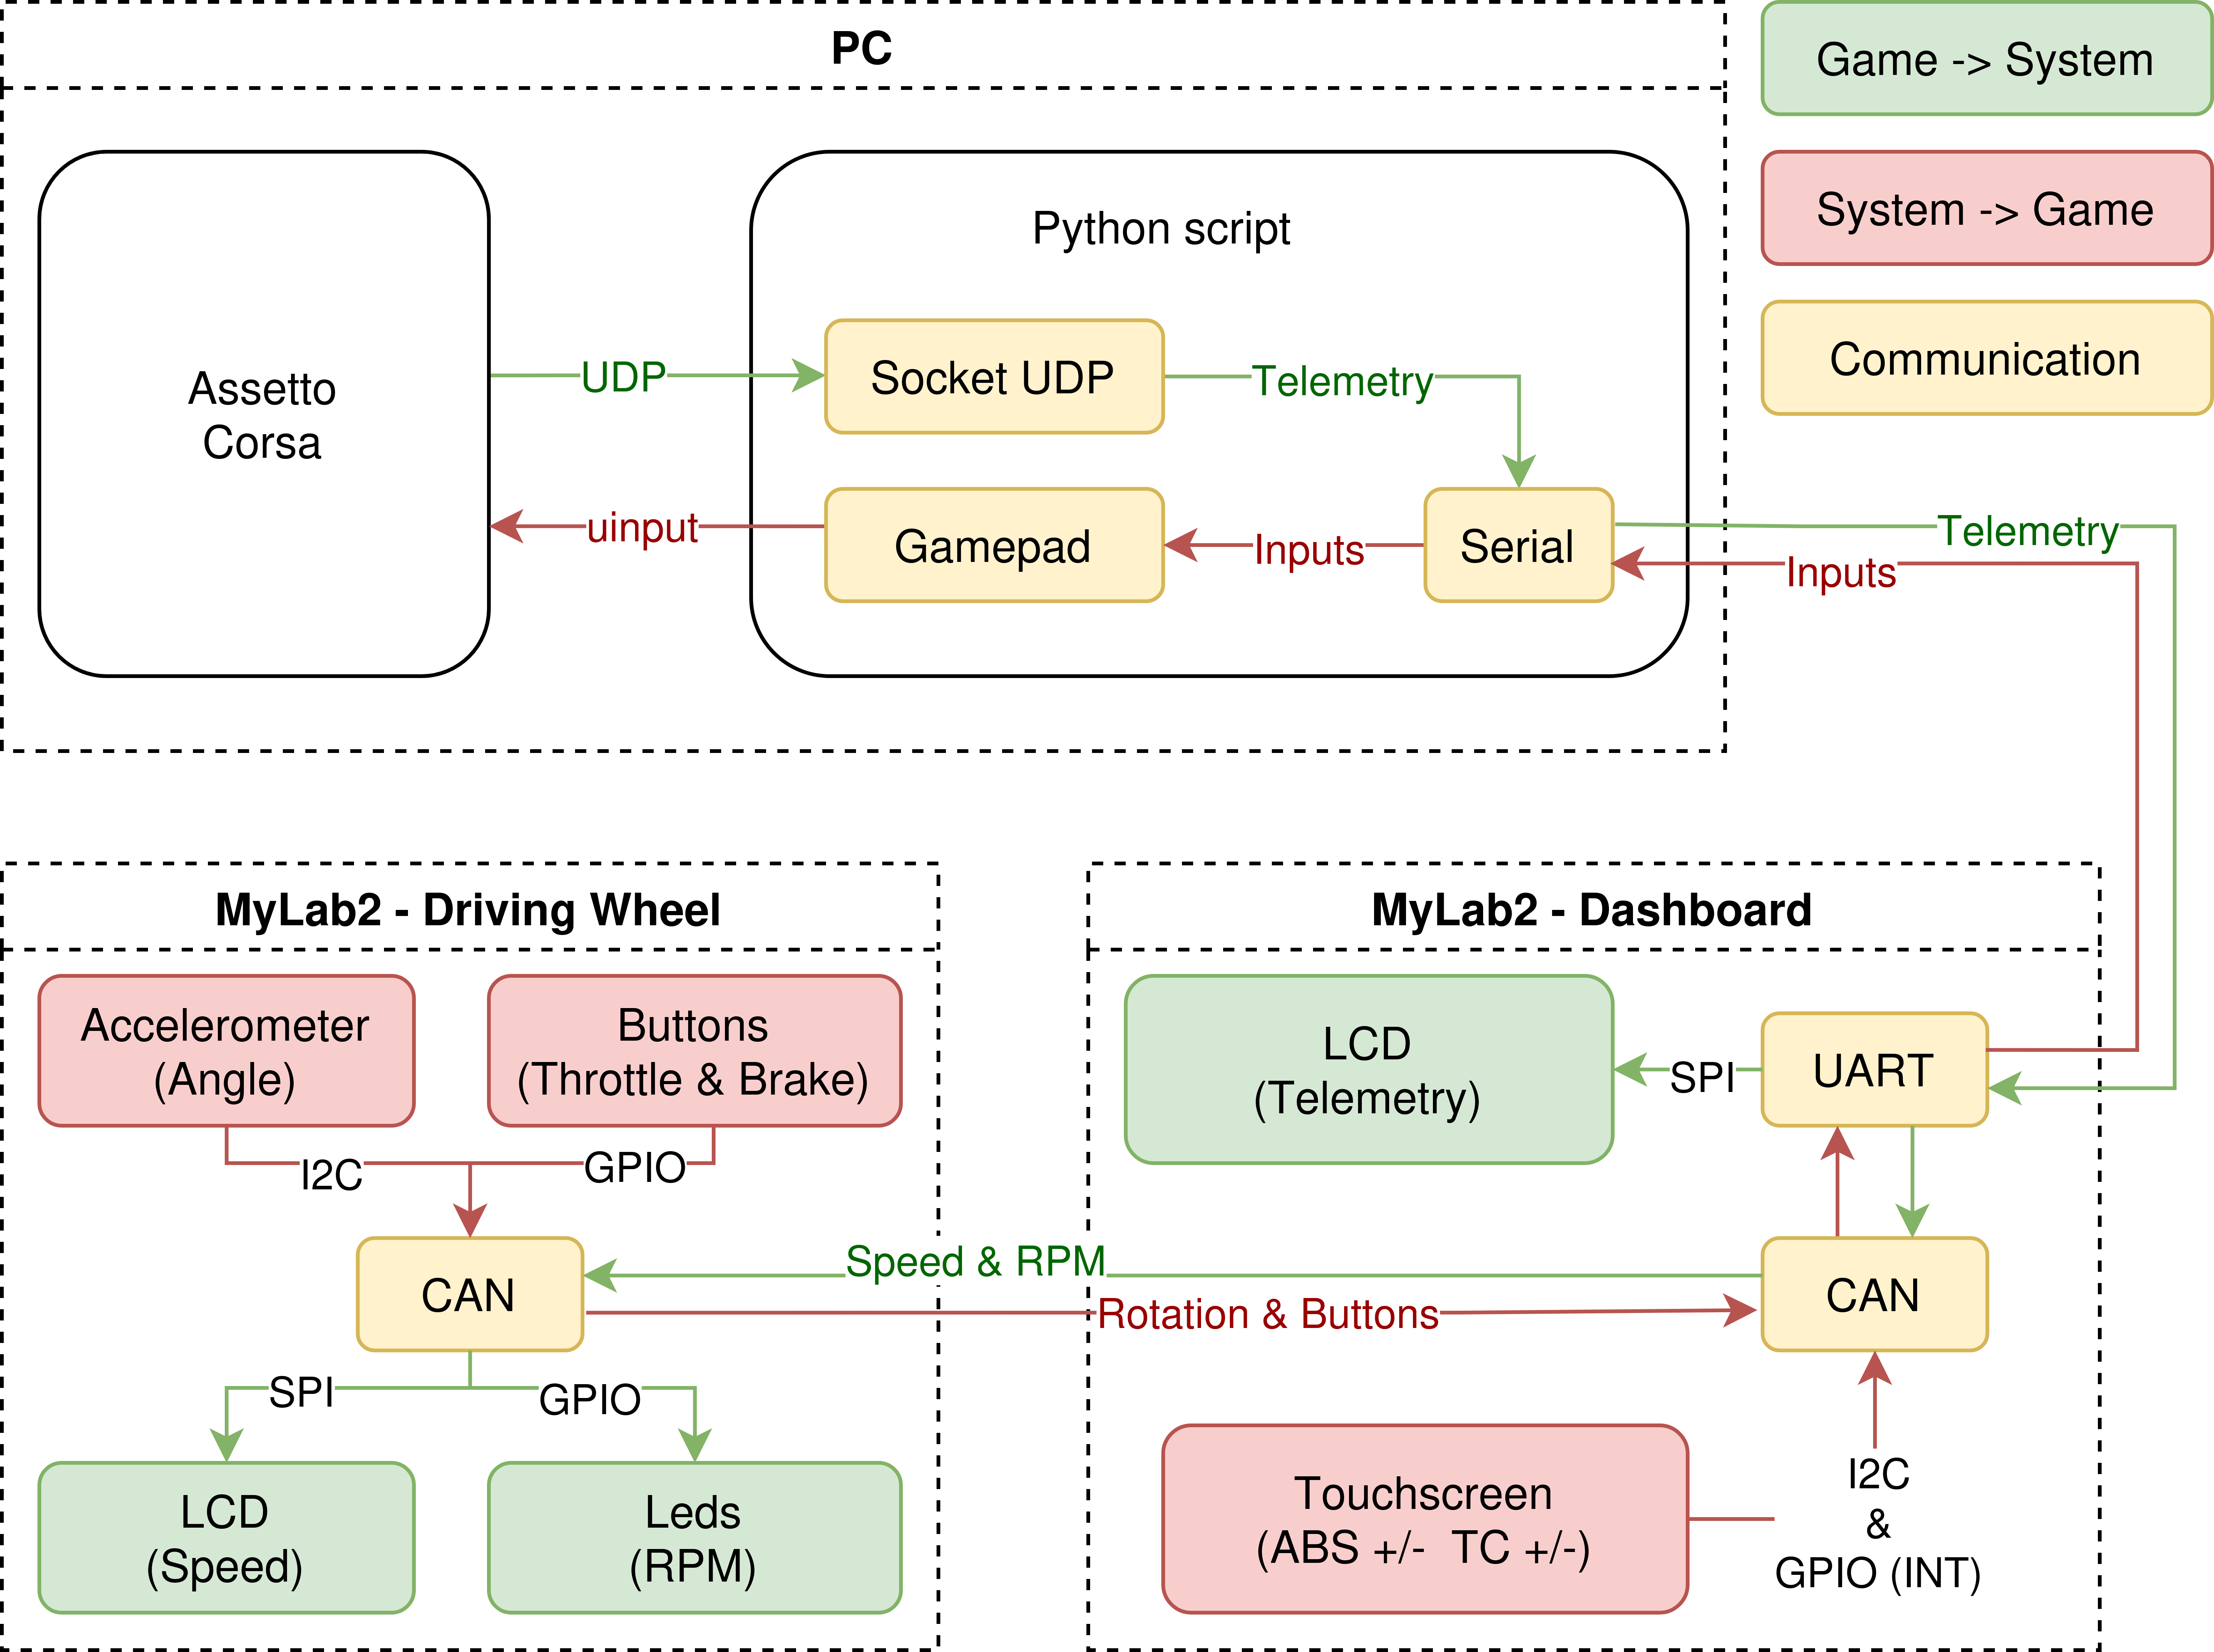
\includegraphics[width=0.7\textwidth]{Images/architecture.drawio.png}
    \end{figure}


\end{frame}


%%%%%%%%%%%%%%%%%%%%%%%%%%%%%%%%%%%%%%%%%%%%%%%%%%%%%%%%%%%%%%%%%%%%%%%%%%%%%%%%%%%%%%%%%%%%%%



\begin{frame}    
    \begin{center}
        \begin{tikzpicture}[remember picture,overlay]
            \node [copy shadow={draw=LightOrange,fill=LightOrange,opacity=0.8,shadow xshift=-0.6ex,
                shadow yshift=-0.6ex},fill=LightYellow,draw=LightYellow,thick,font=\bfseries,anchor=north,inner sep=5pt] at ($(current page.north)-(0cm,0.5cm)$)
                    {\LARGE Problèmes rencontrés};
        \end{tikzpicture}
    \end{center}


    \begin{itemize}[label=\textbullet, leftmargin=1.5cm]
        \item Initialement prévu pour fonctionner avec USB
        \item Installation du jeu -> nécessite une adaptation car jeu Windows
        \item Création des inputs avec python -> ne fonctionne pas chez David
        \item Création d'un profile de contrôles dans le jeu -> ne voulait pas accepter nos inputs 
    \end{itemize}


\end{frame}


%%%%%%%%%%%%%%%%%%%%%%%%%%%%%%%%%%%%%%%%%%%%%%%%%%%%%%%%%%%%%%%%%%%%%%%%%%%%%%%%%%%%%%%%%%%%%%

\begin{frame}    
    \begin{center}
        \begin{tikzpicture}[remember picture,overlay]
            \node [copy shadow={draw=LightOrange,fill=LightOrange,opacity=0.8,shadow xshift=-0.6ex,
                shadow yshift=-0.6ex},fill=LightYellow,draw=LightYellow,thick,font=\bfseries,anchor=north,inner sep=5pt] at ($(current page.north)-(0cm,4cm)$)
                    {\LARGE Démonstration};
        \end{tikzpicture}
    \end{center}

\end{frame}

%%%%%%%%%%%%%%%%%%%%%%%%%%%%%%%%%%%%%%%%%%%%%%%%%%%%%%%%%%%%%%%%%%%%%%%%%%%%%%%%%%%%%%%%%%%%%%

\begin{frame}    
    \begin{center}
        \begin{tikzpicture}[remember picture,overlay]
            \node [copy shadow={draw=LightOrange,fill=LightOrange,opacity=0.8,shadow xshift=-0.6ex,
                shadow yshift=-0.6ex},fill=LightYellow,draw=LightYellow,thick,font=\bfseries,anchor=north,inner sep=5pt] at ($(current page.north)-(0cm,0.5cm)$)
                    {\LARGE Conclusion};
        \end{tikzpicture}
    \end{center}

    \begin{itemize}[label=\textbullet, leftmargin=1.5cm]
        \item Fonctionnel
    \end{itemize}

    \vspace{0.5cm}
    \hspace{0.5cm}\underline{Mais :}
    \normalsize
    \vspace{0.2cm}

    \begin{itemize}[label=\textbullet, leftmargin=1.5cm]
        \item Pas avec les spécifications initiales (USB)
        \item Est peu précis
        \item Nécessité de rendre l'ensemble plus robuste
    \end{itemize}


\end{frame}

%%%%%%%%%%%%%%%%%%%%%%%%%%%%%%%%%%%%%%%%%%%%%%%%%%%%%%%%%%%%%%%%%%%%%%%%%%%%%%%%%%%%%%%%%%%%%%

\begin{frame}    
    \begin{center}
        \begin{tikzpicture}[remember picture,overlay]
            \node [copy shadow={draw=LightOrange,fill=LightOrange,opacity=0.8,shadow xshift=-0.6ex,
                shadow yshift=-0.6ex},fill=LightYellow,draw=LightYellow,thick,font=\bfseries,anchor=north,inner sep=5pt] at ($(current page.north)-(0cm,4cm)$)
                    {\LARGE Questions ?};
        \end{tikzpicture}
    \end{center}

\end{frame}

%%%%%%%%%%%%%%%%%%%%%%%%%%%%%%%%%%%%%%%%%%%%%%%%%%%%%%%%%%%%%%%%%%%%%%%%%%%%%%%%%%%%%%%%%%%%%%

\end{document}